\appendix

\renewcommand{\algorithmicrequire}{\textbf{Input:}}
\newcommand{\deflet}{\textbf{let}}
\newcommand{\mystate}[1]{\STATE \textbf{let} {{}#1}}
\newcommand{\mystop}[1]{\STATE \textbf{stop} \myss{\myangle{{{}#1}}, s'}}
\newcommand{\myss}[1]{${{}#1}$}
\newcommand{\myangle}[1]{\langle {{}#1} \rangle}
\newcommand{\myif}[1]{\IF{\myss{{{}#1}}}}
\newcommand{\myelse}[1]{\ELSIF{\myss{{{}#1}}}}
\newcommand{\SWITCH}[1]{\STATE \textbf{switch} #1\ \textbf{do} \begin{ALC@g}}
\newcommand{\ENDSWITCH}{\end{ALC@g}\STATE \textbf{end switch}}
\newcommand{\CASE}[1]{\STATE \textbf{case} #1\textbf{:} \begin{ALC@g}}
\newcommand{\ENDCASE}{\end{ALC@g}}
\newcommand{\CASELINE}[1]{\STATE \textbf{case} #1\textbf{:} }
\newcommand{\DEFAULT}{\STATE \textbf{default:} \begin{ALC@g}}
\newcommand{\ENDDEFAULT}{\end{ALC@g}}
\newcommand{\DEFAULTLINE}[1]{\STATE \textbf{default:} }




\section{The Security Proofs of UPPRESSO}
\label{ape:model}
We formally analyze  the security properties of UPPRESSO based on the Dolev-Yao style web model as follows.
%which has been widely used in the formal analysis of SSO protocols such as OAuth 2.0~\cite{FettKS16} and OIDC~\cite{FettKS17}.
% ��仰˵�˺ܶ�Σ���appendix�У���ֻ���Ż����ļ�����Ϣ��
We first describe the expressive Dolev-Yao style model of the web infrastructure.
Then,
    we formulate the UPPRESSO system using this model,
        including all entities (i.e., browsers, servers, and scripts) and the transmitted data.
%    present the model of UPPRESSO system, containing normal data and each entities (including browser, servers, and scripts).
%the servers, scripts and the communications among them.
%introduction about how to  indicate the entities (e.g., servers) and communications (e.g., HTTP request) of the web system with Dolev-Yao style web model.
%Then, we describe the model of frequent used data format (e.g., HTTP package) and entity  (e.g., browser).
%Following, we present the modelling UPPRESSO system, containing the servers, scripts and the communications among them.
Finally, we give the security proofs of UPPRESSO, that capture the tracks of all essential data, such as identity token, from its birth to being consumed, to guarantee integrity and confidentiality.



\subsection{The Dolev-Yao Style Web Model}
\label{subsec:webmodel}
Based on Dolev-Yao style model, the web  infrastructure can be modelled as the form of $(\mathcal{W}$, $\mathcal{S}$, $E^0)$. The definitions of these notations is described as below.
\begin{itemize}
\item $\mathcal{W}$ is the set of \textbf{atomic processes}. An atomic process represents an independent entity in the web system, such as browser and web server.
\item $\mathcal{S}$ is the set of \textbf{script processes}. That is, besides the atomic processes in the web system, there are also entities processing data and communicating with other entities, but unable to run independently without other atomic processes. These entities are denoted as script processes, i.e., the JavaScript code in the web system.
\item $E^0$ is the set of self-triggering \textbf{events} initially acceptable to the processes in $\mathcal{W}$. An event is the basic communication elements in the model, representing atomic process A sending a message to atomic process B.
\end{itemize}



\vspace{1mm}
\noindent\textbf{Atomic process}. The atomic process is the modelling web nodes, in the form ($I^p$, $Z^p$, $R^p$, $s_0^p$). The definitions of these notations is described as below.
\begin{itemize}
\item $I^p$ is the set of addresses that the process listens to.
\item  $Z^p$ is the set of \textbf{states} that describes the process. The state is the formal \textbf{term}.
\item $R^p$ is the \textbf{relation} between the input, state $s \in Z^p$ and an event $e$, to the output, the new state $s' \in Z^p$ and an event $e'$. It means that, at one time point, while the process is on state $s$ and receive the event $e$, it would transition to state $s'$ and send the event $e'$ to other process.
\item $s_0^p$ is an initial state.
\end{itemize}

\vspace{1mm}
\noindent\textbf{Term}. Term is the basic element in Dolev-Yao style model, to describe the modelled system.
It contains constants such as ASCII strings and nonce, sequence symbols such as n-ary sequences $\langle \rangle$, $\langle . \rangle$, $\langle . ,. \rangle$, and function symbols that model cryptographic primitives such as $\mathtt{encrypt}, \mathtt{decrypt}$ and digital signatures.
For example, an HTTP request can be modelled as a term containing a type (e.g., $\mathtt{HTTPReq}$), a nonce, a method (e.g., $\mathtt{GET}$ or $\mathtt{POST}$), a domain, a path, URL parameters, request headers and a message body, over the $\Sigma$ in the sequence symbol format. So,
an HTTP GET request for the domain {\sf exa.com/path?para=1} with empty header and body can be described as: $m:=\langle\mathtt{HTTPReq},n,\mathtt{GET},exa.com,/path,\langle \langle para, 1\rangle \rangle ,\langle \rangle,\langle \rangle \rangle$.

\vspace{1mm}
\noindent\textbf{Operations over terms}.
\begin{itemize}
\item \textbf{Equational theory}. Equational theory is defined as usual in Dolev-Yao style models,
 which uses the symbol $\equiv$ to represent the congruence relation on terms, and $\not\equiv$ for non-congruence relation.
 For example, while there are the data $Data$, its signature $Sig$, and the corresponding public key $PubKey$, the relation can be described as $\mathtt{checkSig}(Data, Sig, PubKey)\equiv \mathtt{TRUE}$. 
\item \textbf{Patten Matching}.  We define the term with the variable $*$ as the pattern, such as \myss{\myangle{a, b, *}}.
The pattern matches any term which only replaces the $*$ with other terms. For instance,  \myss{\myangle{a, b, *}} matches \myss{\myangle{a, b, c}}.
\item \textbf{Retrieve attributes from standardized term}. Standardized term is the data in the fixed format, for instance, the HTTP request is the standardized data in the form \myss{\langle\mathtt{HTTPReq}}, \myss{nonce}, \myss{method}, \myss{host}, \myss{path}, \myss{parameters}, \myss{headers}, \myss{body\rangle}.  We assume there is an HTTP request \myss{r :=}  \myss{\langle\mathtt{HTTPReq}},  \myss{n},  \myss{\mathtt{GET}},  \myss{example.com},  \myss{/path},  \myss{\myangle{}},  \myss{\myangle{}},  \myss{\myangle{}\rangle}, here we define the operation on the $r$. That is, the elements in $r$ can be accessed in the form \myss{r.name}, such that \myss{r.method \equiv \mathtt{GET}},  \myss{r.path \equiv /path} and \myss{r.body \equiv \myangle{}}.
\item \textbf{Retrieve attributes from dictionary term}. Dictionary term is the data in the form \myss{\myangle{\myangle{name, value}, \myangle{name, value}, \dotsc}}, for instance the \myss{body} in HTTP request is dictionary data. We assume there is a \myss{body := \myangle{\myangle{username, alice}, \myangle{password, 123}}}, here we define the operation on the $body$. That is, we can access the elements in \myss{body} in the form \myss{body[name]}, such that \myss{body[username] \equiv alice} and \myss{body[password] \equiv 123}. We can also add the new attributes to the dictionary, for example after we set \myss{body[age] := 18}, the \myss{body} are changed into\myss{ \myangle{\myangle{username, alice}, \myangle{password, 123}, \myangle{age, 18}}}.
\end{itemize}

\vspace{1mm}
\noindent\textbf{State}. State is the term consisted of basic terms, to sketch the atomic process at the point of time. For example, the state of a login server can be simplistically described as the term $\langle CookieList,UserList \rangle$, while the $CookieList$ maintains the visitors' cookies with the corresponding login state, and the $UserList$ maintains the user ids and their corresponding passwords.


\vspace{1mm}
\noindent\textbf{Relation}. The relation represents the model of procedure, showing how the entity deal with the received message. For example, while the login server receive the login request from a visitor (the request is denoted as the event $e$), the input of the relation is $e$ and current state $\langle CookieList,UserList \rangle$.   The server verifies the visitor's identity with the $UserList$ and set the login result to $CookieList$ (transitioning to $CookieList'$). Thus the output is the login response $e'$ and the new state $\langle CookieList',UserList \rangle$.


\vspace{1mm}
\noindent\textbf{Script process}. A script process is the modelling JavaScript code, as a relation $R$, representing the server-defined functions, while the input and output are handled by the browser.
To be noticed is that, the script process is addressed by the \verb+Origin+ property, as the the protocol, hostname and port number of a URL. That is, while a script sends the messages to another script process and set the \verb+Origin+ value as the IdP domain, only the script downloaded from IdP server can receive this message.


\vspace{1mm}
\noindent\textbf{Event}. The event  the formal term $\langle a, b, m \rangle$, where $a$ and $b$ represent the addresses of the sender and receiver respectively, and $m$ is the message to be transmitted.





\subsection{The Formulation of UPPRESSO}
In this section, we introduce the model of honest UPPRESSO system, in the form of $(\mathcal{W}$, $\mathcal{S}$, $E^0)$.
$\mathcal{W}$ is the set of atomic processes, including IdP server processes, RP server processes and browsers.
$\mathcal{S}$ is the set of script processes, containing of IdP script process and RP script process.
$E^0$  is the set of events acceptable to the processes in $\mathcal{W}$, which is to be illustrated in the individual processes part.


To be noticed is that, we only focus on the model of servers, browsers and the plain message transmissions among them in this paper, and neglect the HTTPS requests and other necessary Internet facilities (e.g., DNS server) deployed in the UPPRESSO system.
Because we assume that the internet architecture is well  built and HTTPS is well implemented, so that an adversary cannot conduct the attacks targeting these elements.

This section is organized as follows. At first, we introduce the model of normal basic data (representing data in the form of terms), such as HTTP package, which is to be used to construct more complex models.
Then we give the detailed description about the models IdP and RP servers in UPPRESSO system.
At the end, the models of browser and scripts are also introduced.


\subsubsection{Model of Normal Data}
At the very beginning, we provide the modelling normal data, such HTTP messages, used to construct UPPRESSO model.

\vspace{1mm}
\noindent\textbf{HTTP Messages}.
An HTTP request message is the term of the form
\begin{multline*}
\ \ \ \ \ \ \ \ \langle \mathtt{HTTPReq}, nonce, method, host, path, \\
parameters, headers, body\rangle \ \ \ \ \ \ \ \
\end{multline*}
An HTTP response message is the term of the form
\begin{equation*}
    \myangle{\mathtt{HTTPResp}, nonce, status, headers, body}
\end{equation*}
The details are defined as follows:
\begin{itemize}
\setlength\itemsep{-2pt}
 \item \myss{\mathtt{HTTPReq}} and \myss{\mathtt{HTTPResp}} denote the types of messages.
 \item \myss{nonce} is a random number that maps the response to the corresponding request.
 \item \myss{method} is one of the HTTP methods, such as \myss{\mathtt{GET}} and \myss{\mathtt{POST}}.
 \item \myss{host} is the constant string domain of visited server.
 \item \myss{path} is the constant string representing the concrete resource of the server.
 \item \myss{parameters} contains the parameters carried by the url as the form \myss{\myangle{\myangle{name, value}, \myangle{name, value}, \dotsc}}, for example, the \myss{parameters} in the url \myss{http://www.example.com?type=confirm}  is \myss{\myangle{\myangle{type, confirm}}}.
 \item \myss{headers} is the header content of each HTTP messages as the form \myss{\myangle{\myangle{name, value}, \myangle{name, value}, \dotsc}}, such as \myss{\langle\myangle{Referer, http://www.example.com},} \myss{\myangle{Cookies, c}\rangle}.
 \item \myss{body} is the body content carried by HTTP \myss{\mathtt{POST}} request or HTTP response in the form \myss{\myangle{\myangle{name, value}, \myangle{name, value}, \dotsc}}.
  \item \myss{status} is the HTTP status code defined by HTTP standard, such as 200, 302 and 404.
\end{itemize}

\vspace{1mm}\noindent\textbf{URL}.
URL is a term \myss{\myangle{\mathtt{URL}, protocol,host,path,parameters}}, where \myss{\mathtt{URL}} is the type, \myss{protocol} is chosen in \myss{\{\mathtt{S}}, \myss{\mathtt{P}\}} as \myss{\mathtt{S}} stands for HTTPS and \myss{\mathtt{P}} stands for HTTP. The \myss{host, path}, and \myss{parameters} are the same as in HTTP messages.

\vspace{1mm}\noindent\textbf{Origin}.
An Origin is a term \myss{\myangle{host, protocol}} that can represent the server that a script is downloaded from, where \myss{host} and \myss{protocol} are the same as in URL.

\vspace{1mm}\noindent\textbf{POSTMESSAGE}.
PostMessage is used in the browser for transmitting messages between scripts. The postMessage package is defined as the form \myss{\myangle{\mathtt{POSTMESSAGE}, target, Content, Origin}}, where \myss{\mathtt{POSTMESSAGE}} is the type, \myss{target} is the constant nonce which stands for the receiver, \myss{Content} is the message transmitted and \myss{Origin} restricts the receiver's origin.

\vspace{1mm}\noindent\textbf{XMLHTTPREQUEST}.
XMLHTTPRequest is the HTTP message transmitted  by scripts in the browser. That is, the XMLHTTPRequest is converted from the HTTP message by the browser. The XMLHTTPRequest package is defined as the term in the form \myss{\myangle{\mathtt{XMLHTTPREQUEST}, URL, methods, Body, nonce}} can be converted into HTTP request message by the browser, and \myss{\myangle{\mathtt{XMLHTTPREQUEST}, Body, nonce}}  is converted from HTTP response message.

\subsubsection{Models of IdP and RP Servers}
An atomic process is a tuple $p=$ $(I^p, Z^p, R^p,s_0^p )$, containing the addresses, states, and relations.
Here, we will focus on the state form and relation $R$. They can describe that what kind of event can be accepted by the process in each state, and the content of new output events and states.


\vspace{1mm}\noindent\textbf{IdP Server Process}.
The state of IdP server process is described as a term in the form \myss{\myangle{ID, SignKey, sessions, users, RPs, Validity, Tokens}}.
That is,  the state of an IdP server  at the point in time can be sketched using these attributes.
Other data stored at IdP but not used during SSO authentication are not mentioned here.
\begin{itemize}
\setlength\itemsep{-2pt}
\item \myss{ID} is the identifier of IdP.
%\item \myss{p} is the large prime mentioned before.
\item \myss{SignKey} is the private key used by IdP to generate signatures.
\item \myss{sessions} is the term in the form of \myss{\myangle{\myangle{Cookie, session}}}, the Cookie uniquely identifies the session and sessions store the  browser uploaded messages.
\item \myss{users} is the set of user's information, including  \myss{username, password, ID_U}  and other attributes.
\item \myss{RPs} is the set of RP information which consists of ID of RP \myss{(PID_{RP})}, \myss{Endpoints} (i.e., the set of RP's validity endpoints) and \myss{Validity}.
\item \myss{Validity} is the validity for IdP generated signatures.
\item \myss{Tokens} is the set of IdP generated Identity proofs.
\end{itemize}
To make the description clearer, we also provide the \myss{functions} to define the complicated procedure.
\begin{itemize}
\setlength\itemsep{-2pt}
\item \myss{\mathtt{SecretOfID(u)}} is used to search the user \myss{u}'s password.
\item \myss{\mathtt{UIDOfUser(u)}} is used to search the user \myss{u}'s \myss{ID_U}.
\item \myss{\mathtt{ListOfPID()}} is the set of IDs of registered RP.
\item \myss{\mathtt{EndpointsOfRP(r)}} is the set of endpoints registered by the RP with ID \myss{r}.
%\item \myss{\mathtt{ModPow(a, b, c)}} is the result of \myss{a^b \mod c}.
\item \myss{\mathtt{Multiply(P, a)}} is the result of \myss{aP}, where $P$ is the point on elliptic curve and $a$ is the integer.
\item \myss{\mathtt{CurrentTime()}} is the system current time.
\end{itemize}

The relation of IdP process $R^i$ is shown as Relation~\ref{alg1} in Appendix~\ref{ape:alg}.





\vspace{1mm}\noindent\textbf{RP server process}.
The state of RP server process is a term in the form \myss{\myangle{ID_{RP}, Endpoints, IdP, Cert, sessions, users}}. Other attributes are not mentioned here.
\begin{itemize}
\setlength\itemsep{-2pt}
\item \myss{ID_{RP}} and \myss{Endpoints} are RP's registered information at IdP.
\item \myss{Cert} is the IdP signed RP information containing \myss{ID_{RP}, Endpoints} and other attributes.
\item \myss{IdP} is the term of the form \myss{\langle ScriptUrl}, \myss{q}, \myss{PubKey \rangle}, where \myss{ScriptUrl} is the site to download IdP script, \myss{q} is the large prime defined before, and \myss{PubKey} is the public key used to verify the IdP signed messages.
\item \myss{sessions} is same as it in IdP process.
\item \myss{users} is the set of users registered at this RP, each user is uniquely identified by the \myss{Account}.
\end{itemize}

The new \myss{functions} are defined as follows:
\begin{itemize}
\setlength\itemsep{-2pt}
 \item \myss{\mathtt{ExEU}(a, q)} is the Extended Euclidean algorithm, which calculates  \myss{a^{-1} \mod q}.
  \item \myss{\mathtt{Random}()} generates a fresh random number.
  \item \myss{\mathtt{RegisterUser}(Account)} add the new user with \myss{Account} into RP's user list.
\end{itemize}
The relation of RP process $R^r$ is shown as Relation~\ref{alg2} in Appendix~\ref{ape:alg}.


\subsubsection{Model of Browser}
Browser is the essential party in web system, that most of users participates through a browser.
In UPPRESSO, we assume that the browsers are honest and well developed, so that, we neglect  the detailed process of browser, such as constructing and parsing the HTTP package.
Therefore, we only need to analyze how the browsers interactive with other parties in UPPRESSO system.
Moreover, in UPPRESSO system, the message transmitted through a browser is constructing and parsing by the script, so that we only focus on how the script process runs in the browser.

In the browser, a window is the basic unit that shows the content to user.
In a window, the document (Document Object Model, DOM) represents the whole page contained in this window.
The script is one of node in the document.
We introduce the windows and documents of the browser model, which provides inputs and parses the outputs of the script process.
The model of opened windows, documents and downloaded scripts are all the part of state of a browser. For a better reading experience, in this section, we only introduce the model of window and document, and the models of IdP and RP scripts are provided in next section



\vspace{1mm}
\noindent\textbf{Window}. A window \myss{w} is a term of the form \myss{w = \myangle{nonce, documents, opener}}, representing the  the concrete browser window in the system. The \myss{nonce} is the window reference to identify each windows. The \myss{documents} is the set of documents (defined below) including the current document and cached documents (for example, the documents can be viewed via the ``forward" and ``back" buttons in the browser). The \myss{opener} represents the window in which this window is created, for instance, while a user clicks the href in document \myss{d} and it creates a new window \myss{w}, there is \myss{w.opener \equiv d.nonce}.

\vspace{1mm}
\noindent\textbf{Document}. A document \myss{d} is a term of the form
\begin{multline*}
  \ \ \ \langle nonce, location, referrer, script, scriptstate, \\
  scriptinputs, subwindows, active \rangle \ \ \
\end{multline*}
where document is the HTML content in the window.  The \myss{nonce} locates the document. \myss{Location} is the URL where the document is loaded. \myss{Referrer} is same as the Referer header defined in HTTP standard. The \myss{script} is the script process downloaded from each servers. \myss{scriptstate} is define by the script, different in each scripts. The \myss{scriptinputs} is the message transmitted into the script process. The \myss{subwindows} is the set of \myss{nonce} of document's created windows. \myss{active} represents whether this document is active or not.


\subsubsection{Modelling IdP and RP scripts}
The script process is the dependent process relying on the browser, which can be considered as a relation \myss{R} mapping a message input and a message output. And finally the browser will conduct the command in the output message. Here we give the description of the form of input and output.
\begin{itemize}
\setlength\itemsep{-2pt}
\item \textbf{Script Message Input. } The input is the term in the form
\begin{multline*}
\langle tree, docnonce, scriptstate, stateinputs,cookies,\\
localStorage, sessionStorage, ids, secret \rangle
\end{multline*}
\item \textbf{Script Message Output. }The output is the term in the form
\begin{multline*}
\ \ \ \ \ \langle scriptstate, cookies, localStorage, \\
sessionStorage, command \rangle \ \ \ \ \
\end{multline*}
\end{itemize}
The \myss{tree} is the relations of the opened windows and documents, which are visible to this script. \myss{Docnonce} is the document nonce, representing a document. The  \myss{Scriptstate} is a term of the form defined by each script. \myss{Scriptinputs} is the message transmitted to script. However, the \myss{scriptinputs} is defined as standardized forms, for example, postMessage is one of the forms of \myss{scriptinputs}. \myss{Cookies} is the set of cookies that belong to the document's origin. \myss{LocalStorage} is the storage space for browser and \myss{sessionStorage} is the space for each HTTP sessions.  \myss{Ids} is the set of user IDs while \myss{secret} is the password to corresponding user ID. The \myss{command} is the operation which is to be conducted by the browser. Here we only introduce the form of commands used in UPPRESSO system. We have defined the postMessage and XMLHTTPRequest (for HTTP request) message which are the \myss{commands}. Moreover, a term in the form \myss{\myangle{\mathtt{IFRAME}, URL, WindowNonce}} asks the browser to create this document's subwindow and it visits the server with the URL.

\vspace{1mm}
\noindent\textbf{IdP script process}
The state of IdP script process \myss{scriptstate} is a term in the form \myss{\myangle{IdPDomain, Parameters, q, refXHR}}, where
\begin{itemize}
\setlength\itemsep{-2pt}
\item \myss{IdPDomain} is the IdP's host.
\item \myss{Parameters} is used to store the parameters received from other processes.
%\item \myss{p} is the large prime defined before.
\item \myss{q} is used to label the procedure point in the login.
\item \myss{refXHR} is the nonce to map HTTP request and response.
\end{itemize}
The new \myss{functions} are defined as follows.
\begin{itemize}
\setlength\itemsep{-2pt}
 \item \myss{\mathtt{PARENTWINDOW}(tree,docnonce)}. The first parameter is the input relation tree defined before, and the second parameter is the nonce of a document. The output returned by the function is the current window's opener's nonce (null if it doesn't exist nor it is invisible to this document).
  \item \myss{\mathtt{CHOOSEINPUT}(inputs,pattern)}. The first parameter is a set of messages, and the second parameter is a pattern. The result returned by the function is the message in \myss{inputs} matching the \myss{pattern}.
  \item \myss{\mathtt{RandomUrl}()} returns a newly generated host string.
\end{itemize}
The relation of IdP script process $script\_idp$ is shown in Appendix~\ref{ape:alg} Relation~\ref{alg3}.




\vspace{1mm}
\noindent\textbf{RP script process}
The state of RP script process \myss{scriptstate} is a term in the form \myss{\langle IdPDomain}, \myss{RPDomain}, \myss{Parameters}, \myss{q}, \myss{refXHR\rangle}. The \myss{RPDomain} is the host string of the corresponding RP server, and other terms are defined in the same way as in IdP script process.

Here, we define the function \myss{\mathtt{SUBWINDOW}(tree, docnonce)}, which takes the \myss{tree} defined above and the current document's \myss{nonce} as the input. And it selects the \myss{nonce} of the first window opened by this document as the output. However, if there is no opened windows, it returns  null.

The relation of RP script process $script\_rp$ is shown in Appendix~\ref{ape:alg} Relation~\ref{alg4}.

\subsection{Proofs of Security}
In this section, we provide the detailed proof on the security of UPPRESSO. The security definition of UPPRESSO is that the system must ensure only the legitimate user can login to an honest RP under her unique account.
We consider the visits to RP's resource paths are controlled by the visitors' cookies, so that the attacker can break the security only when he owns the cookie bound to the honest user.
However, according to the same origin policy, the cookie is never leaked to any adversary, so the UPPRESSO  system is vulnerable only when a adversary's cookie is bound with the honest user's identity.
Based on the model of RP server process model, at Line 64-83, we can find that only when the RP accept a visitor's token, it would bound this visitor with the identity derived from this token.
Moreover, the RP must also make sure that, an honest user would always login to the server with her constant identity.
Therefore, we can propose the Theorem about the secure UPPRESSO system.
\begin{definition}
%Let $\mathcal{UWS}$ be a UPPRESSO web system, $\mathcal{UWS}$ is secure \textbf{iff} for any honest RP $r$ $\in $ $\mathcal{W}$, it would not derive an honest user's identity from the token while the token belongs to an adversary.
An SSO system is secure \textbf{iff} for any honest RP, it would not derive an honest user's identity from the token while the token belongs to an adversary, or derive an incorrect identity from the token sent by an honest user.
\end{definition}

That is, the requirements of secure SSO system can be described as follows.
\begin{itemize}
\item An adversary cannot achieve an honest user's token issued for an honest RP (\textbf{confidentiality}).
\item An honest RP would not accept the token issued for another RP (\textbf{RP designation}).
\item Attacker cannot forge or modify the IdP-issued proofs (\textbf{integrity}).
\item An honest user must always login to the honest RP on her own identity (\textbf{user identification}).
\end{itemize}

We assume that all the network messages are transmitted using HTTPS, postMessage messages are protected by the browser, and the browsers are  honest, so web attackers can never break the security of UPPRESSO.
Here, we are going to prove that, in the UPRESSO system, the following lemmas are always workable.



\begin{lemma}
An adversary cannot achieve an honest user's token issued for an honest RP (\textbf{confidentiality}).
\label{lemma:confidentiality}
\end{lemma}
\begin{proof}
Here we only need to prove that attackers cannot receive \myss{Token} from other honest processes.
\begin{itemize}
\setlength\itemsep{-2pt}
\item Attacker cannot obtain the \myss{Token} from RP server.  We check all the messages sent by the RP server at Line 4, 7, 19, 25, 31, 36, 45, 55, 61, 66, 74, 84 in Relation~\ref{alg2}. It is easy to prove that the RP server does not send any \myss{Token} to other processes.
\item Attacker cannot obtain the \myss{Token} from RP script. The  messages sent by RP script can be classified into two classes. 1) The messages at Line 18, 36, 56 in Relation~\ref{alg4}  are sent to the RPDomain which is set at Line 4, so that attackers cannot receive these messages. 2) The messages at Line 26,  46 only carry the contents received from RP server, and we have proved that RP server does not send any \myss{Token}. Therefore, attackers cannot receive the \myss{Token} from RP script.
\item Attacker cannot obtain the \myss{Token} from IdP server.  Considering the messages at Line 4, 12, 16, 23, 26, 36, 44, 51, 67 in Relation~\ref{alg1}, we find that only the message at Line 67 carries the \myss{Token}. This \myss{Token} is generated at Line 65, following the trace where the \myss{Content} at Line 63, the \myss{PID_U} at Line 61, the \myss{ID_U} at Line 60, the \myss{session} at Line 48, and finally the \myss{cookie} at Line 47. That is, the receiver of \myss{Token}  must be the owner of the \myss{cookie} in which session that saves the parameter \myss{ID_U} . The \myss{ID_U} is set at Line 15 after verifying the password and never modified. As we assume that passwords cannot be known to attackers,  attackers cannot obtain the \myss{Token} from IdP server.
\item Attacker cannot obtain the \myss{Token} from IdP script. As the proof provided above, only IdP sends the \myss{Token} with the message at Line 67 in Relation~\ref{alg1}, the IdP script can only receive the \myss{Token} at  Line 99 in Relation~\ref{alg3}. Here we are going to prove that the token issued for user $u$'s login to RP $r$ (denoted as \myss{t(u,r)}) can only be  sent to the corresponding RP server through IdP script. The receiver of \myss{t(u,r)} is restricted by the \myss{RPOrigin} at Line 100, which is set at Line 55. The host in the \myss{RPOrigin} is verified using the one included in \myss{Cert} at Line 51. If the \myss{Cert} belong to \myss{r}, the attacker cannot obtain the \myss{t(u,r)}. Now we give the proof that the \myss{Cert} belongs to \myss{r}. Firstly we define the negotiated \myss{PID_{RP}} in \myss{t(u,r)} as \myss{p}. That is the \myss{PID_{RP}} at Line 69 in Relation~\ref{alg2}  must equal to \myss{p} and the \myss{PID_{RP}} is verified at Line 44 with the \myss{RegistrationToken}. This verification cannot be bypassed due to the state check at Line 60. At the same validity period, the IdP script needs to send the registration request with same \myss{p}  and receive the successful registration result. As the IdP checks the uniqueness of \myss{PID_{RP}} at  Line 32 in Relation~\ref{alg1}. The \myss{r} and IdP script must share the same \myss{RegistrationToken}. As the \myss{RegistrationToken} contains the \myss{\mathtt{Hash}(N_U)}, the IdP script and \myss{r} must share the same \myss{ID_{RP}}. Therefore, the  \myss{Cert} saved as the IdP scriptstate parameter must belong to \myss{r}.
\end{itemize}
Therefore, attackers cannot  learn users' valid identity proofs.
\end{proof}


\begin{lemma}
An honest RP would not accept the token issued for another RP (\textbf{RP designation}).
\label{lemma:RPdesignation}
\end{lemma}
\begin{proof}
We can find that an RP server finally accept the $PID_U$ in an token at Line 77 in Relation~\ref{alg2}, after the verification at Line 73. The $PID_{RP}$ retrieved at Line 69, must be verified at Line 44.
The content verified at Line 44 is received from IdP server, generated at Line 41, Relation~\ref{alg1} and protected by the signature generated at Line 42.
According to the verification at 32, the content containing $PID_{RP}$ is unique during the valid time.
Moreover, according to Line 42, 44 (the $N_U$ used at Line 42 is set  at  Line 15, used for generating $PID_{RP}$ at Line 13), the $PID_{RP}$ must be resigned for this RP, as no other RP cannot generate the same $PID_{RP}$ with this $N_U$.
As it has been proved at Lemma~\ref{lemma:confidentiality}, an malicious RP cannot receive the valid token issued for another RP, therefore, the adversary would not receive the token including an honest RP's $PID_{RP}$ from honest user.
\end{proof}


\begin{lemma}
Attacker cannot forge or modify the IdP-issued proofs (\textbf{integrity}).
\label{lemma:integrity}
\end{lemma}
\begin{proof}
The IdP-issued proofs include the \myss{Cert} used in \myss{script\_idp}, the \myss{RegistrationResult} and \myss{Token} used in \myss{P^r} . We can easily find that the IdP does not send the private key to any processes so that the attackers cannot obtain the private key. Then we only need to prove that all the proofs are well verified.
\begin{itemize}
\setlength\itemsep{-2pt}
\item \myss{Cert} is used at Line 21, 52 in Relation~\ref{alg3}. At Line 21, the \myss{Cert} has already been verified at Line 16. At Line 52, the \myss{Cert} is picked from the state parameters, and the cert parameter is set at Line 19.  At Line 19, the \myss{Cert} has already been verified at Line 16.
At Line 16 the \myss{Cert} is verified with the public key in the scriptstate, where the key is considered initially honest and the key is not modified at Relation~\ref{alg3}. Therefore, \myss{Cert} cannot be forged or modified.
\item \myss{RegistrationResult} is used in Relation~\ref{alg2} from Line 35 to 55, which is verified at Line 30. The public key is initially set in the RP and never modified. Therefore, \myss{RegistrationResult} cannot be forged or modified.
\item \myss{Token} is used in Relation~\ref{alg2} from Line 69 to 84 after Line 65 where it is verified.  As proved before, the public key is honestly set and never modified. Therefore, \myss{Token} cannot be forged or modified.
\end{itemize}
Therefore, this lemma is proved.
\end{proof}


\begin{lemma}
An honest user must always login to the honest RP on her own identity (\textbf{user identification}).
\label{lemma:userIdentification}
\end{lemma}
\begin{proof}
We can find that, the RP accepts the user's identity at Line 83, Relation~\ref{alg2}. And the identity is generated at Line 79, based on the $PID_U$  retrieved from the token and the trapdoor $t^{-1}$.
The $t^{-1}$ is generated at Line 14, set at Line 17, and never changed, as the multiplicative inverse of $N_U$.
According to Lemma~\ref{lemma:integrity}, only the IdP can generate an token, so that the token must be issued at Line 65, Relation~\ref{alg1}.
IdP generates the $PID_U$ based on the $PID_{RP}$ and user's $ID_U$.
According to Lemma~\ref{lemma:RPdesignation}, while the $PID_{RP}$ is accepted by an RP, the $PID_{RP}$ must be the generated between the RP and user.
According to Lemma~\ref{lemma:confidentiality}, the $ID_U$ must belongs to the honest user.
Therefore, the user's identity must equal with the constant $ [ID_U]ID_{RP}$.

Moreover, an adversary may lead the honest user to upload the adversary's token to an RP.
While the honest user has already negotiated the $PID_{RP}$ with the RP.
The opener of the IdP script must be the RP script.
As the $N_U$ generated at Line 7, Relation~\ref{alg3}, and $PID_{RP}$ generated at Line 21, Relation~\ref{alg3} and Line 13, Relation~\ref{alg2}.
The $t$ is only sent to RP script at Line 8, Relation~\ref{alg3}, and RP server at Line 18, Relation~\ref{alg4}.
The $PID_{RP}$ is only sent to IdP server at Line 28 and 90, Relation~\ref{alg3}. Moreover, the registration result including the $PID_{RP}$ is sent to IdP script at Line  36, Relation~\ref{alg1}, RP script at Line 40, Relation~\ref{alg3}, RP server at Line 36, Relation~\ref{alg4}. An adversary can never know the $PID_{RP}$ negotiated between the honest user and RP.
While the honest user has not negotiated the $PID_{RP}$ with the RP yet, the \verb+session+[$PID_{RP}$] at Line 69, Relation~\ref{alg2} and other similar attributes must be empty, as the $Cookie$ used at Line 58 belongs to the honest user and the negotiation between Line 10-20 does not conducted by the user.
Therefore, an adversary cannot lead the honest RP to accept the malicious token from the honest user.
\end{proof}

In conclusion, four lemmas prove that the UPPRESSO system satisfies the requirements of the secure SSO system.
Therefore, the following theorem is proved.
\begin{theorem}
UPPRESSO is the secure SSO system.
\end{theorem}






\onecolumn

\section{Relations}
\label{ape:alg}
Relation takes an event and a state as input and returns a new state and a sequence of events.
In a web system,
     it represents how the entities, such as the server, deal with the received messages, and send message to other entities.
This section provides the detailed relations of the processes (including atomic and script processes) in UPPRESSO.


\subsection{IdP process}
The IdP process only accepts the events, downloading scripts, accessing the login status of a cookie owner, authenticating with password, registering the $PID_{RP}$, and requiring the identity token.
The detailed procedure of dealing with these events is shown as follows.

\begin{breakablealgorithm}
  \caption{\textbf{IdP\_Process\_Relation}}
  \label{alg1}
  \begin{algorithmic}[1]
  \REQUIRE \myss{\myangle{a, b, m}, s}
  \mystate{\myss{s':=s}}
  \mystate{\myss{n, method, path, parameters, headers, body} \textbf{such that}}\\
  \ \ \myss{\myangle{\mathtt{HTTPReq},n,method,path,parameters,headers,body} \equiv m}\\
  \ \ \textbf{if} \myss{possible}; \textbf{otherwise} stop \myss{\myangle{}, s'}
  \myif{path \equiv /script}
  \mystate{\myss{m':=\myangle{\mathtt{HTTPResp},n,200, \myangle{}, \mathtt{IdPScript}}}}
  \mystop{f, a, m'}
  \myelse{path \equiv /login}
  \mystate{\myss{cookie := headers[Cookie]}}
  \mystate{\myss{session := s'.sessions[cookie]}}
  \mystate{\myss{username:=body[username]}}
  \mystate{\myss{password:=body[password]}}
  \myif{password \not\equiv \mathtt{SecretOfID}(username)}
  \mystate{\myss{m' :=\myangle{\mathtt{HTTPResp},n,200,\myangle{},\mathtt{LoginFailure}}}}
  \mystop{b, a,m'}
  \ENDIF
  \mystate{\myss{session[uid] := \mathtt{UIDOfUser}(username)}}
  \mystate{\myss{m' :=\myangle{\mathtt{HTTPResp},n,200,\myangle{},\mathtt{LoginSucess}}}}
  \mystop{b, a,m'}
  \myelse{path \equiv /loginInfo}
  \mystate{\myss{cookie := headers[Cookie]}}
  \mystate{\myss{session := s'.sessions[cookie]}}
  \mystate{\myss{username := session[username]}}
  \myif{username \not\equiv \mathtt{null}}
  \mystate{\myss{m' := \myangle{\mathtt{HTTPResp},n,200,\myangle{},\mathtt{Logged}}}}
  \mystop{b, a,m'}
  \ENDIF
  \mystate{\myss{m' := \myangle{\mathtt{HTTPResp},n,200,\myangle{},\mathtt{Unlogged}}}}
  \mystop{b, a,m'}
  \myelse{path \equiv /dynamicRegistration}
  \mystate{\myss{PID_{RP} := body[PID_{RP}]}}
 \mystate{\myss{Endpoint := body[Endpoint]}}
  \mystate{\myss{Nonce := body[Nonce]}}
  \myif{PID_{RP} \in \mathtt{ListOfPID()}}
  \mystate{\myss{Content :=\myangle{Fail, PID_{RP}, Nonce}}}
  \mystate{\myss{Sig := \mathtt{Sig}(Content, s'.SignKey)}}
  \mystate{\myss{RegistrationResult := \myangle{Content, Sig}}}
  \mystate{\myss{m' := \myangle{\mathtt{HTTPResp}, n, 200, \myangle{}, RegistrationResult}}}
  \mystop{b, a,m'}
  \ENDIF
  \mystate{\myss{Validity := \mathtt{CurrentTime} ()+ s'.Validity}}
 \mystate{\myss{s'.RPs := s'.RPs +  ^{\myangle{}} \myangle{PID_{RP}, Endpoint, Validity}}}
  \mystate{\myss{Content := \myangle{OK, PID_{RP}, Nonce, Validity}}}
  \mystate{\myss{Sig := \mathtt{Sig}(Content, s'.SignKey)}}
  \mystate{\myss{RegistrationResult := \myangle{Content, Sig}}}
  \mystate{\myss{m' := \myangle{\mathtt{HTTPResp}, n, 200, \myangle{}, RegistrationResult}}}
  \mystop{b, a,m'}
  \myelse{path \equiv /authorize}
  \mystate{\myss{cookie := headers[Cookie]}}
  \mystate{\myss{session := s'.sessions[cookie]}}
  \mystate{\myss{username := session[username]}}
  \myif{username \equiv \mathtt{null}}
  \mystate{\myss{m' := \myangle{\mathtt{HTTPResp}, n, 200, \myangle{}, \mathtt{Fail}}}}
  \mystop{b, a,m'}
  \ENDIF
  \mystate{\myss{PID_{RP} := parameters[PID_{RP}]}}
  \mystate{\myss{Endpoint := parameters[Endpoint]}}
  \myif{PID_{RP} \notin \mathtt{ListOfPID}() \lor Endpoint \notin \mathtt{EndpointsOfRP}(PID_{RP})}
  \mystate{\myss{m' := \myangle{\mathtt{HTTPResp}, n, 200, \myangle{}, \mathtt{Fail}}}}
  \mystop{b, a,m'}
  \ENDIF
  \mystate{\myss{ID_U := session[uid]}}
  \mystate{\myss{PID_U := \mathtt{Multiply}(PID_{RP}, ID_U)}}
  \mystate{\myss{Validity := \mathtt{CurrentTime} ()+ s'.Validity}}
  \mystate{\myss{Content := \myangle{PID_{RP}, PID_U, s'.ID, Validity}}}
  \mystate{\myss{Sig := \mathtt{Sig}(Content, s'.SignKey)}}
  \mystate{\myss{Token := \myangle{Content, Sig}}}
  \mystate{\myss{s'.Tokens := s'.Tokens + ^{\myangle{}}Token}}
  \mystate{\myss{m' := \myangle{\mathtt{HTTPResp}, n, 200, \myangle{}, \myangle{Token, Token}}}}
  \mystop{f, a, m'}
  \ENDIF
  \mystop{}
  \end{algorithmic}
\end{breakablealgorithm}


\subsection{RP process}
The RP process only accepts the events, downloading scripts, redirecting to IdP server, negotiating the $PID_{RP}$, uploading the $PID_{RP}$ registration result and identity token.
The detailed procedure of dealing with these events is shown as follows.
\begin{breakablealgorithm}
  \caption{\textbf{RP\_Process\_Relation}}
  \label{alg2}
  \begin{algorithmic}[1]
  \REQUIRE \myss{\myangle{a, b, m}, s}
  \mystate{\myss{s:=s'}}
  \mystate{\myss{n, method, path, parameters, headers, body} \textbf{such that}}\\
  \ \ \myss{\myangle{\mathtt{HTTPReq},n,method,path,parameters,headers,body} \equiv m}\\
  \ \ \textbf{if} \myss{possible}; \textbf{otherwise} stop \myss{\myangle{}, s'}
  \myif{path \equiv /script}
\mystate{\myss{m':=\myangle{\mathtt{HTTPResp},n,200, \myangle{}, \mathtt{RPScript}}}}
  \mystop{f, a, m'}
  \myelse{path \equiv /login}
  \mystate{\myss{m'  := \myangle{\mathtt{HTTPResp},n,302,\myangle{\myangle{Location, s'.IdP.ScriptUrl}}, \myangle{}}}}
  \mystop{f, a, m'}
  \myelse{path \equiv /startNegotiation}
  \mystate{\myss{cookie := headers[Cookie]}}
  \mystate{\myss{session := s'.sessions[cookie]}}
  \mystate{\myss{t := parameters[t]}}
  \mystate{\myss{PID_{RP} := \mathtt{Multiply}(s'.ID_{RP}, t)}}
  \mystate{\myss{t^{-1}:= \mathtt{ExEU}(t, s'.IdP.q)}}
  \mystate{\myss{session[t] := t}}
  \mystate{\myss{session[PID_{RP}] := PID_{RP}}}
  \mystate{\myss{session[t^{-1}] := t^{-1}}}
  \mystate{\myss{session[state] := expectRegistration}}
  \mystate{\myss{m' := \myangle{\mathtt{HTTPResp}, n, 200, \myangle{}, \myangle{Cert, s'.Cert}}}}
 \mystop{f, a, m'}
 \myelse{path \equiv /registrationResult}
 \mystate{\myss{cookie := headers[Cookie]}}
  \mystate{\myss{session := s'.sessions[cookie]}}
  \myif{session[state] \not\equiv expectRegistration}
  \mystate{\myss{m' := \myangle{\mathtt{HTTPResp}, n, 200, \myangle{}, \mathtt{Fail}}}}
  \mystop{f, a, m'}
  \ENDIF
  \mystate{\myss{RegistrationResult := body[RegistrationResult]}}
  \mystate{\myss{Content:=RegistrationResult.Content}}
  \myif{\mathtt{checksig}(Content, RegistrationResult.Sig, s'.IdP.PubKey) \equiv \mathtt{FALSE}}
  \mystate{\myss{m' := \myangle{\mathtt{HTTPResp}, n, 200, \myangle{}, \mathtt{Fail}}}}
  \mystate{\myss{session := \mathtt{null}}}
  \mystop{f, a, m'}
  \ENDIF
  \myif{Content.Result \not\equiv OK}
  \mystate{\myss{m' := \myangle{\mathtt{HTTPResp}, n, 200, \myangle{}, \mathtt{Fail}}}}
  \mystate{\myss{session := \mathtt{null}}}
  \mystop{f, a, m'}
  \ENDIF
  \mystate{\myss{PID_{RP} := session[PID_{RP}]}}
  \mystate{\myss{t := session[t]}}
  \mystate{\myss{Nonce := \mathtt{Hash}( t)}}
  \mystate{\myss{Time := \mathtt{CurrentTime}()}}
  \myif{PID_{RP} \not\equiv Content.PID_{RP} \lor Nonce \not\equiv Content.Nonce \lor Time > Content.Validity}
  \mystate{\myss{m' := \myangle{\mathtt{HTTPResp}, n, 200, \myangle{}, \mathtt{Fail}}}}
  \mystate{\myss{session := \mathtt{null}}}
  \mystop{f, a, m'}
  \ENDIF
  \mystate{\myss{session[PIDValidity] := Content.Validity}}
  \mystate{\myss{Endpoint \in s'.Endpoints}}
  \mystate{\myss{session[state] := expectToken}}
  \mystate{\myss{Nonce' := \mathtt{Random}()}}
  \mystate{\myss{session[Nonce] := Nonce'}}
  \mystate{\myss{Body := \myangle{PID_{RP}, Endpoint, Nonce'}}}
  \mystate{\myss{m' := \myangle{\mathtt{HTTPResp}, n, 200, \myangle{}, Body}}}
  \mystop{f, a, m'}
  \myelse{path \equiv /uploadToken}
 \mystate{\myss{cookie := headers[Cookie]}}
  \mystate{\myss{session := s'.sessions[cookie]}}
  \myif{session[state] \not\equiv expectToken}
  \mystate{\myss{m' := \myangle{\mathtt{HTTPResp}, n, 200, \myangle{}, \mathtt{Fail}}}}
  \mystop{f, a, m'}
  \ENDIF
  \mystate{\myss{Token := body[Token]}}
  \myif{\mathtt{checksig}(Token.Content, Token.Sig, s'.IdP.PubKey) \equiv \mathtt{FALSE}}
  \mystate{\myss{m' := \myangle{\mathtt{HTTPResp}, n, 200, \myangle{}, \mathtt{Fail}}}}
  \mystop{f, a, m'}
  \ENDIF
  \mystate{\myss{PID_{RP} := session[PID_{RP}]}}
  \mystate{\myss{Time := \mathtt{CurrentTime}()}}
  \mystate{\myss{PIDValidity := session[PIDValidity]}}
  \mystate{\myss{Content := Token.Content}}
  \myif{PID_{RP} \not\equiv Content.PID_{RP} \lor Time>Content.Validity \lor Time>PIDValidity}
  \mystate{\myss{m' := \myangle{\mathtt{HTTPResp}, n, 200, \myangle{}, \mathtt{Fail}}}}
  \mystop{f, a, m'}
  \ENDIF
  \mystate{\myss{PID_U := Content.PID_U}}
  \mystate{\myss{t^{-1} := session[t^{-1}]}}
  \mystate{\myss{Account := \mathtt{Multiply}(PID_U, t^{-1})}}
  \myif{Account \in \mathtt{ListOfUser}()}
  \mystate{\myss{\mathtt{RegisterUser}(Account)}}
  \ENDIF
  \mystate{\myss{session[user] := Account}}
  \mystate{\myss{m' := \myangle{\mathtt{HTTPResp}, n, 200, \myangle{}, \mathtt{LoginSuccess}}}}
  \mystop{f, a, m'}
  \ENDIF
  \mystop{}
  \end{algorithmic}
\end{breakablealgorithm}


\subsection{IdP script process}
The IdP script process accepts the events,
(a) self-triggering events  for starting $PID_{RP}$ negotiation;
(b) the postMessage from other scripts for sending the $Cert$, and request of identity token;
(c) the HTTP response for transmitting registration result and identity token.
The detailed procedure of dealing with these events is shown as follows.

\begin{breakablealgorithm}
  \caption{\textbf{IdP\_Script\_Relation}}
  \label{alg3}
  \begin{algorithmic}[1]
  \REQUIRE \myss{\myangle{tree, docnonce, scriptstate, scriptinputs, cookies, localStorage, sessionStorage, ids, secret}}
  \mystate{\myss{ s' := scriptstate}}
  \mystate{\myss{command := \myangle{}}}
  \mystate{\myss{target := \mathtt{PARENTWINDOW}(tree,docnonce)}}
  \mystate{\myss{IdPDomain := s'.IdPDomain}}
  \SWITCH{\myss{s'.q}}
    \CASE{\myss{start}}
      \mystate{\myss{t := \mathtt{Random}()}}
      \mystate{\myss{command := \myangle{\mathtt{POSTMESSAGE}, target, \myangle{\myangle{t, t}}, \mathtt{null}}}}
      \mystate{\myss{s'.Parameters[t] := t}}
      \mystate{\myss{s'.q := expectCert}}
    \ENDCASE
    \CASE{\myss{expectCert}}
      \mystate{\myss{pattern := \myangle{\mathtt{POSTMESSAGE}, *, Content, *}}}
      \mystate{\myss{input := \mathtt{CHOOSEINPUT}(scriptinputs,pattern)}}
      \myif{input \not\equiv \mathtt{null}}
      \mystate{\myss{Cert := input.Content[Cert]}}
      \myif{\mathtt{checksig}(Cert.Content, Cert.Sig, s'.PubKey) \equiv \mathtt{null}}
      \mystate{\myss{\textbf{stop}\ \myangle{}}}
      \ENDIF
       \mystate{\myss{s'.Parameters[Cert] := Cert}}
      \mystate{\myss{t := s'.Parameters[t]}}
      \mystate{\myss{PID_{RP} := \mathtt{Multiply}(Cert.Content.ID_{RP}, t)}}
      \mystate{\myss{s'.Parameters[PID_{RP}] := PID_{RP}}}
      \mystate{\myss{Endpoint := \mathtt{RandomUrl}()}}
      \mystate{\myss{s'.Parameters[Endpoint] := Endpoint}}
      \mystate{\myss{Nonce := \mathtt{Hash}(t)}}
      \mystate{\myss{Url := \myangle{\mathtt{URL}, \mathtt{S}, IdPDomain, /dynamicRegistration,\myangle{} }}}
      \mystate{\myss{s'.refXHR :=  \mathtt{Random}()}}
      \mystate{\myss{command : = \langle\mathtt{XMLHTTPREQUEST}, Url, \mathtt{POST},} \\\ \ \ \ \myss{ \myangle{\myangle{PID_{RP}, PID_{RP}}, \myangle{Nonce, Nonce}, \myangle{Endpoint, Endpoint}}, s'.refXHR\rangle}}
      \mystate{\myss{s'.q := expectRegistrationResult}}
       \ENDIF
      \ENDCASE
      \CASE{expectRegistrationResult}
      \mystate{\myss{pattern := \myangle{\mathtt{XMLHTTPREQUEST},Body,s'.refXHR}}}
      \mystate{\myss{input := \mathtt{CHOOSEINPUT}(scriptinputs,pattern) }}
      \myif{input \not\equiv \mathtt{null} \land input.Content[RegistrationResult].type \equiv OK}
      \mystate{\myss{RegistrationResult := input.Body[RegistrationResult]}}
      \myif{ RegistrationResult.Content.Result \not\equiv OK}
      \mystate{\myss{s'.q := stop}}
      \mystate{\myss{\textbf{stop}\ \myangle{}}}
      \ENDIF
      \mystate{\myss{command := \myangle{\mathtt{POSTMESSAGE}, target, \myangle{\myangle{RegistrationResult, RegistrationResult}}, \mathtt{null}}}}
      \mystate{\myss{s'.q := expectProofRquest}}
      \ENDIF
      \ENDCASE
      \CASE{expectProofRquest}
      \mystate{\myss{pattern := \myangle{\mathtt{POSTMESSAGE}, *, Content, *}}}
      \mystate{\myss{input := \mathtt{CHOOSEINPUT}(scriptinputs,pattern)}}
      \myif{input \not\equiv \mathtt{null}}
       \mystate{\myss{PID_{RP} := input.Content[PID_{RP}]}}
       \mystate{\myss{Endpoint_{RP} := input.Content[Endpoint]}}
       \mystate{\myss{s'.Parameters[Nonce] := input.Content[Nonce]}}
       \mystate{\myss{Cert := s'.Parameters[Cert]}}
      \myif{Endpoint_{RP} \notin Cert.Content.Endpoints \lor PID_{RP} \not\equiv s'.Parameters[PID_{RP}]}
      \mystate{\myss{s'.q := stop}}
      \mystate{\myss{\textbf{stop}\ \myangle{}}}
      \ENDIF
       \mystate{\myss{s'.Parameters[Endpoint_{RP}] := Endpoint_{RP}}}
      \mystate{\myss{Url := \myangle{\mathtt{URL}, \mathtt{S}, IdPDomain, /loginInfo, \myangle{}}}}
      \mystate{\myss{s'.refXHR :=  \mathtt{Random}()}}
      \mystate{\myss{command : = \myangle{\mathtt{XMLHTTPREQUEST}, Url, \mathtt{GET},\myangle{}, s'.refXHR}}}
      \mystate{\myss{s'.q := expectLoginState}}
      \ENDIF
      \ENDCASE
      \CASE{expectLoginState}
      \mystate{\myss{pattern := \myangle{\mathtt{XMLHTTPREQUEST},Body,s'.refXHR}}}
      \mystate{\myss{input := \mathtt{CHOOSEINPUT}(scriptinputs,pattern) }}
      \myif{input \not\equiv \mathtt{null}}
      \myif{input.Body \equiv \mathtt{Logged}}
      \mystate{\myss{username \in ids}}
      \mystate{\myss{Url := \myangle{\mathtt{URL}, \mathtt{S}, IdPDomain, /login, \myangle{}}}}
     \ mystate{\myss{s'.refXHR :=  \mathtt{Random}()}}
      \mystate{\myss{command : = \myangle{\mathtt{XMLHTTPREQUEST}, Url, \mathtt{POST},\myangle{\myangle{username, username}, \myangle{password, secret}}, s'.refXHR}}}
      \mystate{\myss{s'.q := expectLoginResult}}
      \myelse{input.Body \equiv \mathtt{Unlogged}}
      \mystate{\myss{PID_{RP} := s'.Parameters[PID_{RP}]}}
      \mystate{\myss{Endpoint := s'.Parameters[Endpoint]}}
      \mystate{\myss{Nonce := s'.Parameters[Nonce]}}
      \mystate{\myss{Url := \langle \mathtt{URL}, \mathtt{S}, IdPDomain, /authorize,}\\\ \ \ \  \myss{\myangle{\myangle{PID_{RP}, PID_{RP}}, \myangle{Endpoint, Endpoint}, \myangle{Nonce, Nonce}} \rangle}}
      \mystate{\myss{s'.refXHR :=  \mathtt{Random}()}}
      \mystate{\myss{command : = \myangle{\mathtt{XMLHTTPREQUEST}, Url, \mathtt{GET},\myangle{}, s'.refXHR}}}
      \mystate{\myss{s'.q := expectToken}}
      \ENDIF
      \ENDIF
      \ENDCASE
      \CASE{expectLoginResult}
      \mystate{\myss{pattern := \myangle{\mathtt{XMLHTTPREQUEST},Body,s'.refXHR}}}
      \mystate{\myss{input := \mathtt{CHOOSEINPUT}(scriptinputs,pattern) }}
      \myif{input \not\equiv \mathtt{null}}
      \myif{input.Body \not\equiv \mathtt{LoginSuccess}}
      \mystate{\myss{\textbf{stop}\ \myangle{}}}
      \ENDIF
      \mystate{\myss{PID_{RP} := s'.Parameters[PID_{RP}]}}
      \mystate{\myss{Endpoint := s'.Parameters[Endpoint]}}
      \mystate{\myss{Nonce := s'.Parameters[Nonce]}}
      \mystate{\myss{Url := \langle \mathtt{URL}, \mathtt{S}, IdPDomain, /authorize,}\\\ \ \ \  \myss{\myangle{\myangle{PID_{RP}, PID_{RP}}, \myangle{Endpoint, Endpoint}, \myangle{Nonce, Nonce}} \rangle}}
      \mystate{\myss{s'.refXHR :=  \mathtt{Random}()}}
      \mystate{\myss{command : = \myangle{\mathtt{XMLHTTPREQUEST}, Url, \mathtt{GET},\myangle{}, s'.refXHR}}}
      \mystate{\myss{s'.q := expectToken}}
      \ENDIF
      \ENDCASE
      \CASE{expectToken}
      \mystate{\myss{pattern := \myangle{\mathtt{XMLHTTPREQUEST},Body,s'.refXHR}}}
      \mystate{\myss{input := \mathtt{CHOOSEINPUT}(scriptinputs,pattern) }}
      \myif{input \not\equiv \mathtt{null}}
      \mystate{\myss{Token := input.Body[Token]}}
      \mystate{\myss{RPOringin := \myangle{s'.Parameters[Endpoint_{RP}], \mathtt{S}}}}
      \mystate{\myss{command := \myangle{\mathtt{POSTMESSAGE},target,\myangle{Token,Token},RPOrigin}}}
      \mystate{\myss{s .q := stop}}
     \ENDIF
    \ENDCASE
  \ENDSWITCH
\mystate{\myss{\textbf{stop}\ \myangle{s',cookies,localStorage,sessionStorage,command}}}
    \end{algorithmic}
\end{breakablealgorithm}


\subsection{RP script process}
The RP script process accepts the events,
(a) self-triggering events  for opening the new window;
(b) the postMessage from other scripts for $PID_{RP}$ negotiation, posting registration result and identity token;
(c) the HTTP response for downloading the RP $Cert$, retrieving identity token request and confirming login result.
The detailed procedure of dealing with these events is shown as follows.

\begin{breakablealgorithm}
  \caption{\textbf{RP\_Script\_Relation}}
  \label{alg4}
  \begin{algorithmic}[1]
\REQUIRE \myss{\myangle{tree, docnonce, scriptstate, scriptinputs, cookies, localStorage, sessionStorage, ids, secret}}
\mystate{\myss{ s' := scriptstate}}
  \mystate{\myss{command := \myangle{}}}
  \mystate{\myss{IdPWindow := \mathtt{SUBWINDOW}(tree,docnonce).nonce}}
  \mystate{\myss{RPDomain := s'.RPDomain}}
  \mystate{\myss{IdPOringin := \myangle{s'.IdPDomian, \mathtt{S}}}}
  \SWITCH{\myss{s'.q}}
    \CASE{\myss{start}}
    \mystate{\myss{Url := \myangle{\mathtt{URL}, \mathtt{S}, RPDomain, /login, \myangle{}}}}
    \mystate{\myss{command := \myangle{\mathtt{IFRAME}, Url, \_SELF}}}
    \mystate{\myss{s'.q := expectt}}
    \ENDCASE
    \CASE{\myss{expectt}}
    \mystate{\myss{pattern := \myangle{\mathtt{POSTMESSAGE}, *, Content, *}}}
      \mystate{\myss{input := \mathtt{CHOOSEINPUT}(scriptinputs,pattern)}}
      \myif{input \not\equiv \mathtt{null}}
      \mystate{\myss{t := input.Content[t]}}
      \mystate{\myss{Url := \myangle{\mathtt{URL}, \mathtt{S}, RPDomain, /startNegotiation, \myangle{}}}}
      \mystate{\myss{s'.refXHR :=  \mathtt{Random}()}}
      \mystate{\myss{command : = \myangle{\mathtt{XMLHTTPREQUEST}, Url, \mathtt{POST},\myangle{\myangle{t, t}}, s'.refXHR}}}
      \mystate{\myss{s'.q := expectCert}}
      \ENDIF
      \ENDCASE
      \CASE{\myss{expectCert}}
      \mystate{\myss{pattern := \myangle{\mathtt{XMLHTTPREQUEST},Body,s'.refXHR}}}
      \mystate{\myss{input := \mathtt{CHOOSEINPUT}(scriptinputs,pattern) }}
      \myif{input \not\equiv \mathtt{null}}
      \mystate{\myss{Cert := input.Content[Cert]}}
      \mystate{\myss{command := \myangle{\mathtt{POSTMESSAGE}, IdPWindow, \myangle{\myangle{Cert, Cert}}, IdPOringin}}}
      \mystate{\myss{s'.q := expectRegistrationResult}}
      \ENDIF
      \ENDCASE
      \CASE{\myss{expectRegistrationResult}}
      \mystate{\myss{pattern := \myangle{\mathtt{POSTMESSAGE}, *, Content, *}}}
      \mystate{\myss{input := \mathtt{CHOOSEINPUT}(scriptinputs,pattern)}}
      \myif{input \not\equiv \mathtt{null}}
      \mystate{\myss{RegistrationResult := input.Content[RegistrationResult]}}
      \mystate{\myss{Url := \myangle{\mathtt{URL}, \mathtt{S}, RPDomain, /registrationResult, \myangle{}}}}
      \mystate{\myss{s'.refXHR :=  \mathtt{Random}()}}
      \mystate{\myss{command : = \myangle{\mathtt{XMLHTTPREQUEST}, Url, \mathtt{POST},\myangle{\myangle{RegistrationResult, RegistrationResult}}, s'.refXHR}}}
      \mystate{\myss{s'.q := expectTokenRequest}}
      \ENDIF
      \ENDCASE
      \CASE{\myss{expectTokenRequest}}
      \mystate{\myss{pattern := \myangle{\mathtt{XMLHTTPREQUEST},Body,s'.refXHR}}}
      \mystate{\myss{input := \mathtt{CHOOSEINPUT}(scriptinputs,pattern) }}
      \myif{input \not\equiv \mathtt{null}}
      \mystate{\myss{PID_{RP} := input.Content.Body[PID_{RP}]}}
      \mystate{\myss{Endpoint := input.Content.Body[Endpoint]}}
      \mystate{\myss{Nonce := input.Content.Body[Nonce]}}
      \mystate{\myss{command := \langle\mathtt{POSTMESSAGE}, IdPWindow}, \\\ \ \ \  \myss{\myangle{\myangle{PID_{RP}, PID_{RP}}, \myangle{Endpoint, Endpoint}, \myangle{Nonce, Nonce}},  IdPOringin\rangle}}
      \mystate{\myss{s'.q := expectToken}}
      \ENDIF
      \ENDCASE
      \CASE{\myss{expectToken}}
      \mystate{\myss{pattern := \myangle{\mathtt{POSTMESSAGE}, *, Content, *}}}
      \mystate{\myss{input := \mathtt{CHOOSEINPUT}(scriptinputs,pattern)}}
      \myif{input \not\equiv \mathtt{null}}
      \mystate{\myss{Token := input.Content[Token]}}
      \mystate{\myss{Url := \myangle{\mathtt{URL}, \mathtt{S}, RPDomain, /uploadToken, \myangle{}}}}
      \mystate{\myss{s'.refXHR :=  \mathtt{Random}()}}
      \mystate{\myss{command : = \myangle{\mathtt{XMLHTTPREQUEST}, Url, \mathtt{POST},\myangle{\myangle{Token, Token}}, s'.refXHR}}}
      \mystate{\myss{s'.q := expectLoginResult}}
      \ENDIF
      \ENDCASE
      \CASE{\myss{expectLoginResult}}
      \mystate{\myss{pattern := \myangle{\mathtt{XMLHTTPREQUEST},Body,s'.refXHR}}}
      \mystate{\myss{input := \mathtt{CHOOSEINPUT}(scriptinputs,pattern) }}
      \myif{input \not\equiv \mathtt{null}}
      \myif{input.Body \equiv \mathtt{LoginSuccess}}
      \mystate{\myss{LoadHomepage}}
      \ENDIF
      \ENDIF
    \ENDCASE
    \ENDSWITCH
\end{algorithmic}
\end{breakablealgorithm}


\begin{comment}
\section{Privacy Analysis}
\label{sec:privacy}


In this section, we will give the privacy proof and show that UPPRESSO is secure against both IdP-based login tracing and RP-based identity linkage attacks.

\noindent\textbf{IdP-based login tracing.}
As shown in figure~\ref{fig:process}, the only information that is related to the RP's identity and is accessible to the IdP is $PID_{RP}$, which is converted from $ID_{RP}$ using a random $t$. Since $t$ is randomly chosen from $\mathbb{Z}_n$ by the user and the IdP ha no control of the process, the IdP should treat $PID_{RP}$ as being randomly chosen from $\mathbb{G}$. So, the IdP cannot recognize the RP nor derive its real identity. Therefore, IdP-based identity linkage becomes impossible in UPPRESSO.

Next, we will prove that UPPRESSO prevents RP-based identity linkage based on the Decisional Diffie-Hellman (DDH) assumption~\cite{GoldwasserK16}. Here, we briefly introduce the DDH assumption:
%\noindent\textbf{The DDH Assumption.}
Let $q$ be a large prime and $\mathbb{G}$ denotes a cyclic group of order $n$ of an elliptic curve $E(\mathbb{F}_q)$.
Assume that $n$ is also a large prime. Let $P$ be a generator point of $\mathbb{G}$. The DDH assumption for $\mathbb{G}$ states that for any probabilistic polynomial time (PPT) algorithm $D$, the two probability distributions \{$aP$, $bP$, $abP$\} and \{$aP$, $bP$, $cP$\}, where $a$, $b$, and $c$ are randomly and independently chosen from $\mathbb{Z}_n$, are computationally indistinguishable in the sense that there is a negligible $\sigma(n)$ with the security parameter $n$ such that:
%where $q$ and $n$ are large primitive number, and $P$ is the point of $\mathbb{G}$.
%For any probabilistic polynomial time (PPT) algorithm $D$, the distributions, \{$P$, $aP$, $bP$, $abP$\}$_{a,b \in \mathbb{Z}_n}$ and \{$P$, $aP$, $bP$, $cP$\}$_{a,b,c \in \mathbb{Z}_n}$, are computationally indistinguishable. There is a negligible $\sigma(k)$, where $k$ is the security parameter.
\vspace{-\topsep}
\begin{multline*}
Pr[D(P, aP, bP, abP)=1]-Pr[D(P, aP, bP, cP)=1]=\sigma(n)
\end{multline*}
\vspace{-\topsep}

\vspace{-2mm}
\noindent\textbf{RP-based identity linkage.}
Collusive RPs can act arbitrarily to correlate $PID_U$s at different RPs and guess if they belong to the same user. Therefore, we consider the collusive RPs are playing a guessing Game. In this Game, the IdP and the users act as the challenger, while the collusive RPs act as the adversary (denoted as $A$ in Figure~\ref{fig:game}). RP-based identity linkage is impossible in UPPRESSO {\em if and only if the adversary has no advantage over the challenger in the guessing game.}


\vspace{1mm}
\begin{strip}
\centering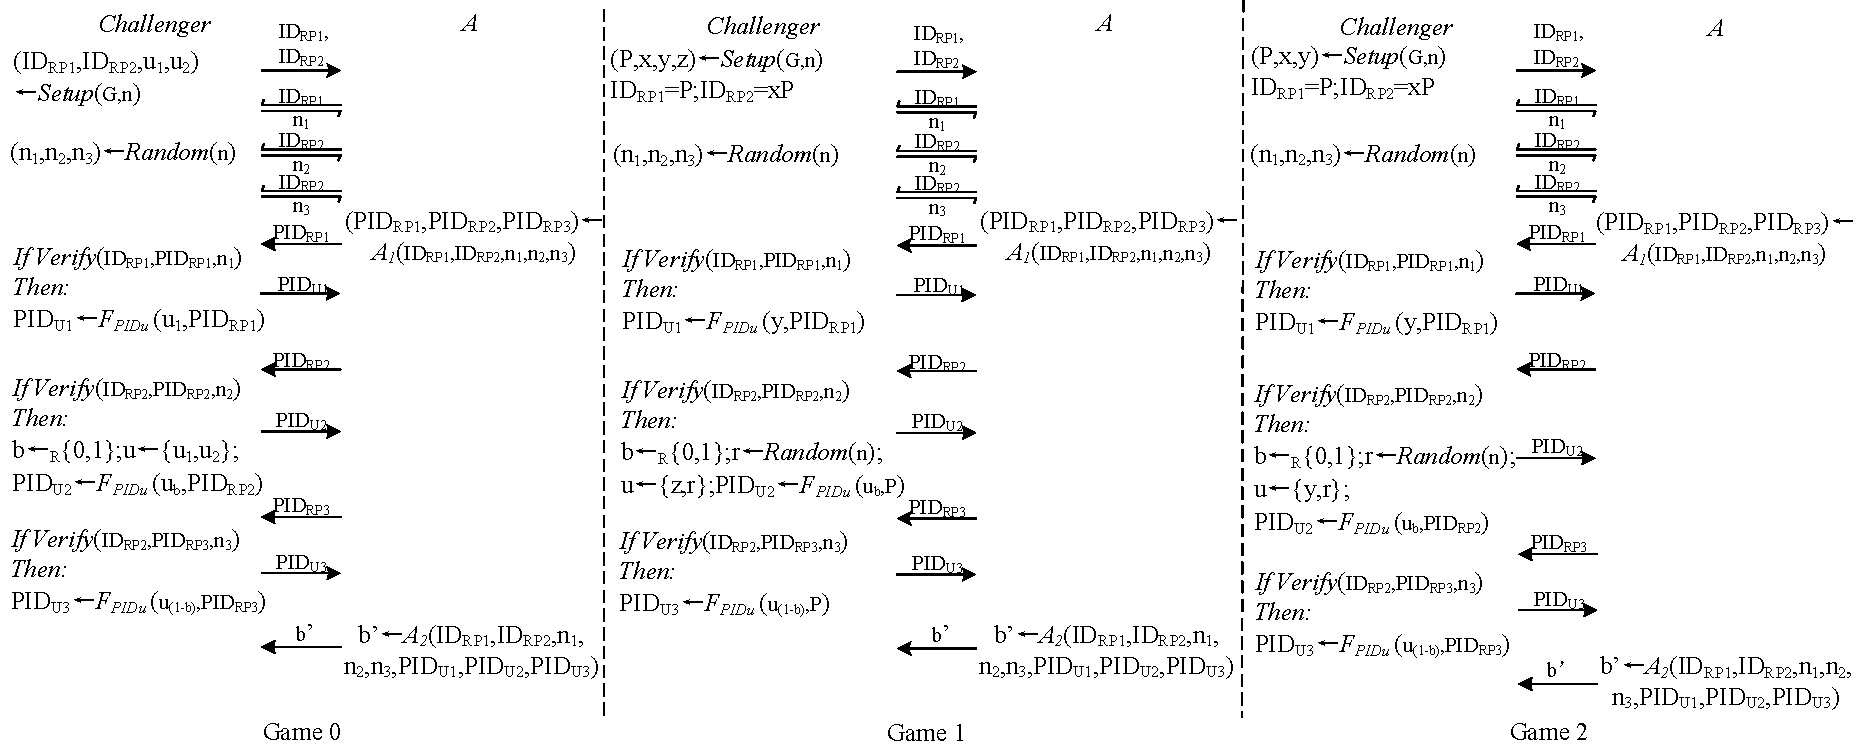
\includegraphics[width=\textwidth, height=0.35\textheight]{fig/game.pdf}
\captionof{figure}{Interactions between the challenger and the adversary in three Games.}
\label{fig:game}
\vspace{-5mm}
\end{strip}


Next, we model the guessing Game to depict the interactions between the challenger and the adversary. First, we describe the challenger's actions in the Game as follows.
\begin{itemize}
\vspace{-\topsep}
\item[-] {\em Initialization:} In initialization, the challenger generates $ID_{RP}$s and $ID_U$s for multiple RPs and users using the initialization algorithm $Setup(G,n)$, where $G$ and $n$ are defined in table~\ref{tbl:notations}.
\vspace{-\topsep}
\item[-] {\em Random number generation:} When the challenger receives the $ID_{RP}$s from the adversary, it generates a random $t \in \mathbb{Z}_n$ for each $ID_{RP}$ using the algorithm $Random(n)$. %$t$ will be used to generate the corresponding $PID_{RP}$.
\vspace{-\topsep}
\item[-] {\em $PID_U$ generation:} When the challenger receives an $PID_{RP}$, it first verifies if the $PID_{RP}$ is generated for $ID_{RP}$ with the corresponding $t$, using the algorithm $Verify(ID_{RP},PID_{RP},t)$. Then, it generates the $PID_U$ with the algorithm $F_{PID_U}(ID_U,PID_{RP})$ and sends it to the adversary.
%\vspace{-\topsep}
\end{itemize}

To prove the privacy of UPPRESSO against RP-based identity linkage, we define three Games, as shown in figure~\ref{fig:game}. First, based on the above description, we model the $ID_U$-guessing game following the UPPRESSO design as $\mathtt{Game 0}$ : (1) First, the adversary receives two $ID_{RP}$s (i.e., $ID_{RP1}$ and $ID_{RP2}$) and three $t$s (i.e., $n_1$, $n_2$, and $n_3$). It then generates three $PID_{RP}$s accordingly. From the challenger's view, three $PID_{RP}$s are related to three $t$s, respectively. (2) Then, the challenger generates $PID_U$s for different $PID_{RP}$s, using two $ID_U$s (i.e., $u_1$ and $u_2$). %generated in the initialization phase.
In particular, the challenger generates $PID_{U1}$ from $ID_{U1}$ directly, and selects a random number $b \in \{0, 1\}$ to generate $PID_{U2}=ID_{Ub} \cdot PID_{RP2}$, and $PID_{U3}=ID_{U(1-b)} \cdot PID_{RP3}$. (3) Finally, the adversary sends its guess $b'$ to the challenger. If $b'=b$, the adversary wins the game.

We define the event [$b'=b$] in $\mathtt{Game 0}$ as $\Gamma$. If the adversary has no advantage in guessing $b$ correctly, which indicates the $PID_U$s are generated from the same $ID_U$, the probability $Pr[\Gamma]$ should be 1/2. Therefore, we conclude that in $\mathtt{Game 0}$, UPPRESSO is secure against RP-based identity linkage if and only if $Pr[\Gamma]=1/2$.


Next, we build the ideal model of the guessing game, denoted as $\mathtt{Game 1}$. In this model, the probability that the adversary correctly guessing $b$ is 1/2. This time, the challenger randomly selects $z$ and $r$ and uses them to generate $PID_{U2}$ and $PID_{U3}$, respectively. Since the adversary does not know $z$ and $r$, he does not know $b$ neither. Similarly, we define the event [$b'=b$] in $\mathtt{Game 1}$ as $\Gamma_1$, and $Pr[\Gamma_1]$ should be 1/2.

According to the DDH assumption, we need to prove that $|Pr[\Gamma_1]-Pr[\Gamma]|=\sigma(n)$, where $\sigma(n)$ is negligible. So, we build another model of Game, denoted as $\mathtt{Game 2}$, by setting the values of the parameters defined in $\mathtt{Game 0}$ to be: $ID_{RP2}=xID_{RP1}$, $u_1=y$ and $u_2=r$, where $r$ is a random number. Again, we define the event [$b'=b$] in  $\mathtt{Game 2}$ as $\Gamma_2$, and $Pr[\Gamma_2]=Pr[\Gamma]$ should be true.

After defining the three games, we prove that $|Pr[\Gamma_1]-Pr[\Gamma_2]|=\sigma(n)$ as follows. In each game, the adversary uses the algorithm $A_2$ to derive $b'$ from the collected data, i.e., $\{ID_{RP1},ID_{RP2},n_1,n_2,n_3,PID_{U1},PID_{U2},PID_{U3}\}$. Now, let us replace the parameters in $\mathtt{Game 1}$ and $\mathtt{Game 2}$ with the exact values:
\vspace{-\topsep}
\begin{equation*}
\begin{aligned}
    b'_{game1} \gets A_2(P,xP,n_1,n_2,n_3,yn_1P,zP,rP) \\
    b'_{game2}\gets A_2(P,xP,n_1,n_2,n_3,yn_1P,xyn_2P,rn_3P) \\
    or \; b'_{game2}\gets A_2(P,xP,n_1,n_2,n_3,yn_1P,rn_2P,xyn_3P)
\end{aligned}
\end{equation*}
\vspace{-\topsep}

Since $n_1$, $n_2$, $n_3$ are randomly chosen by the challenger, which are not related to $ID_U$, the adversary can easily remove them and obtain $b'_{game1}\gets A_2(P,xP,yP,zP,rP)$ in $\mathtt{Game 1}$ and $b'_{game2}\gets A_2(P,xP,yP,xyP,xrP)$ in $\mathtt{Game 2}$.

As $r$ is randomly chosen and unknown to the adversary, $rP$ and $xrP$ are also random points. We can re-write $b'_{game1}$ and $b'_{game2}$ as $b'_{game1}\gets A_2(P,xP,yP,zP,r_1P)$ and $b'_{game2}\gets A_2(P,xP,yP,xyP,r_2P)$, which means there is no non-negligible difference between the success probability in $\mathtt{Game 1}$ and $\mathtt{Game 2}$, according to the DDH assumption. Otherwise, we should be able to build a PPT distinguishing algorithm that breaks DDH assumption about the adversary.

Such distinguishing algorithm $D$ is shown in figure~\ref{fig:dalgorithm}.
The inputs of the algorithm is $\{P,X,Y,Z\}$. To the adversary, it is $\mathtt{Game 1}$ if the input is in the form $\{P,xP,yP,zP\}_{x,y,z \in \mathbb{Z}_n}$, and it is $\mathtt{Game 1}$ if the input is $\{P,xP,yP,xyP\}_{x,y \in \mathbb{Z}_n}$. As a result,
\vspace{-\topsep}
\begin{multline*}
   \ \ \ \ \ \ \ \ \ \ \ \ \ \ \ \ \  Pr[D(P,xP,yP,zP)=1]=Pr[{\Gamma_1}]\\
   Pr[D(P,xP,yP,xyP)=1]=Pr[{\Gamma_2}]\ \ \ \ \ \ \ \ \ \ \ \ \ \ \ \ \ \
\end{multline*}

\vspace{-\topsep}
Therefore, $|Pr[\Gamma_1]-Pr[\Gamma_2]|=\sigma(n)$, where $\sigma(n)$ is negligible, and $n$ is the security parameter. It means the adversary has no advantage in guessing $b$ in $\mathtt{Game 0}$. Therefore, he cannot distinguish if two $PID_U$s at two different RPs belong to the same user or not. This proves that UPPRESSO is resistant to RP-based identity linkage attacks.

\end{comment}


\begin{comment}
\begin{figure}[t]
  \centering
  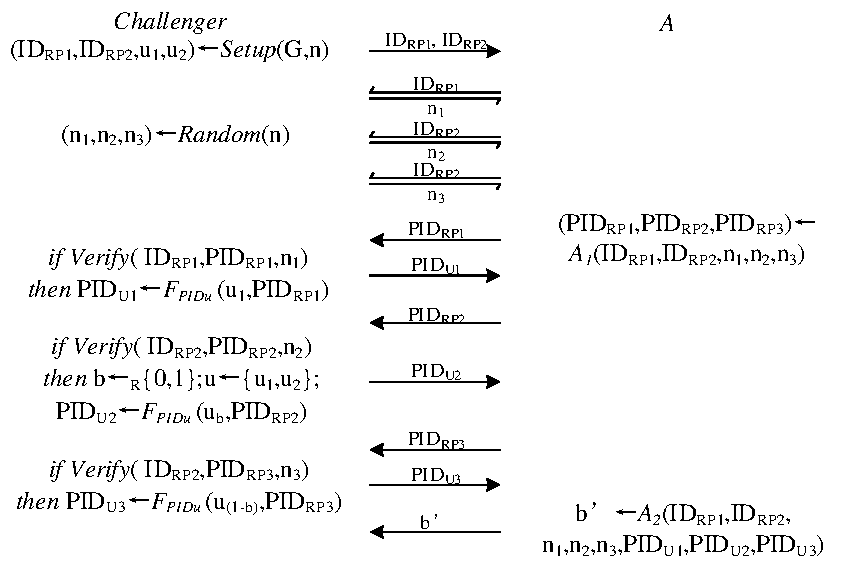
\includegraphics[width=1\linewidth]{fig/game0.pdf}
  \vspace{-5mm}
  \caption{Game 0.}
  \label{fig:game0}
  \vspace{-5mm}
\end{figure}


\begin{figure}[t]
  \centering
  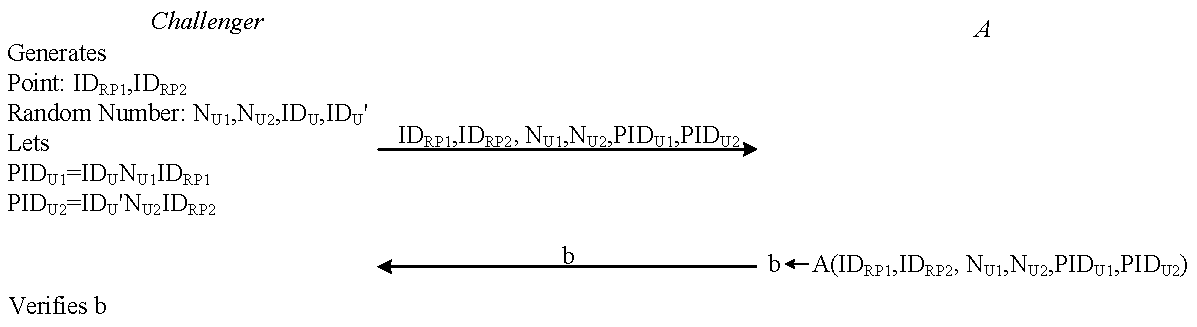
\includegraphics[width=1\linewidth]{fig/game1.pdf}
  \vspace{-5mm}
  \caption{Game 1.}
  \label{fig:game1}
    \vspace{-5mm}
\end{figure}

\begin{figure}[t]
  \centering
  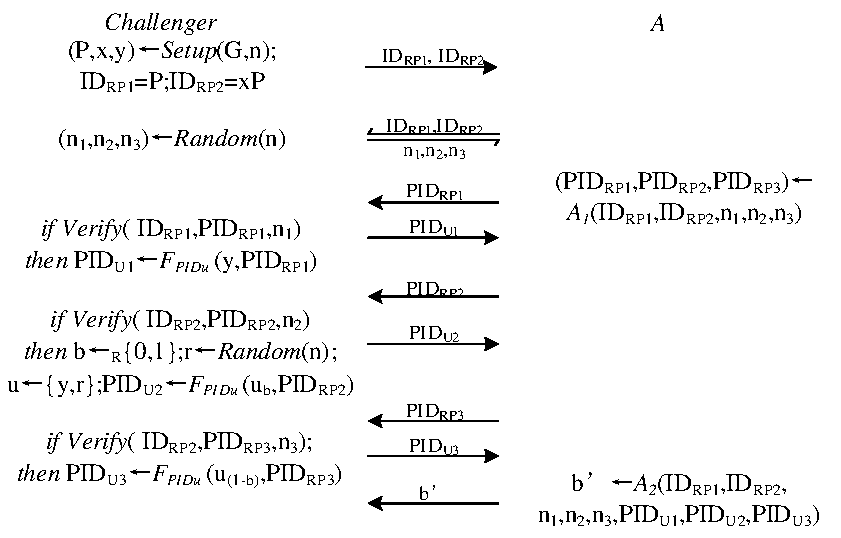
\includegraphics[width=1\linewidth]{fig/game2.pdf}
  \vspace{-5mm}
  \caption{Game 2.}
  \label{fig:game2}
  \vspace{-5mm}
\end{figure}

\end{comment}

%\end{appendices}
